\label{sec:dslam}
As illustraded in \Cref{fig:sysframe} there are tow main inter-robot components in DSLAM system: 1) place recognition and matching. 2) inter-robot relative pose (RelPose) estimation. In this section we implement these components both based on submaps.

\subsection{Submap-Based Place Recognition}
The key problem of place recognition is to extrct discriminative feature vector from 2D submap.

\subsection{Submap-Based RelPose Estimation}
% Because submap contains the position of the map at the single-robot trajectory, the RelPose of two robots can be estimated by calculating the pose of two submaps in the same scene, which is well defined as map registration.

\begin{figure}[t]
    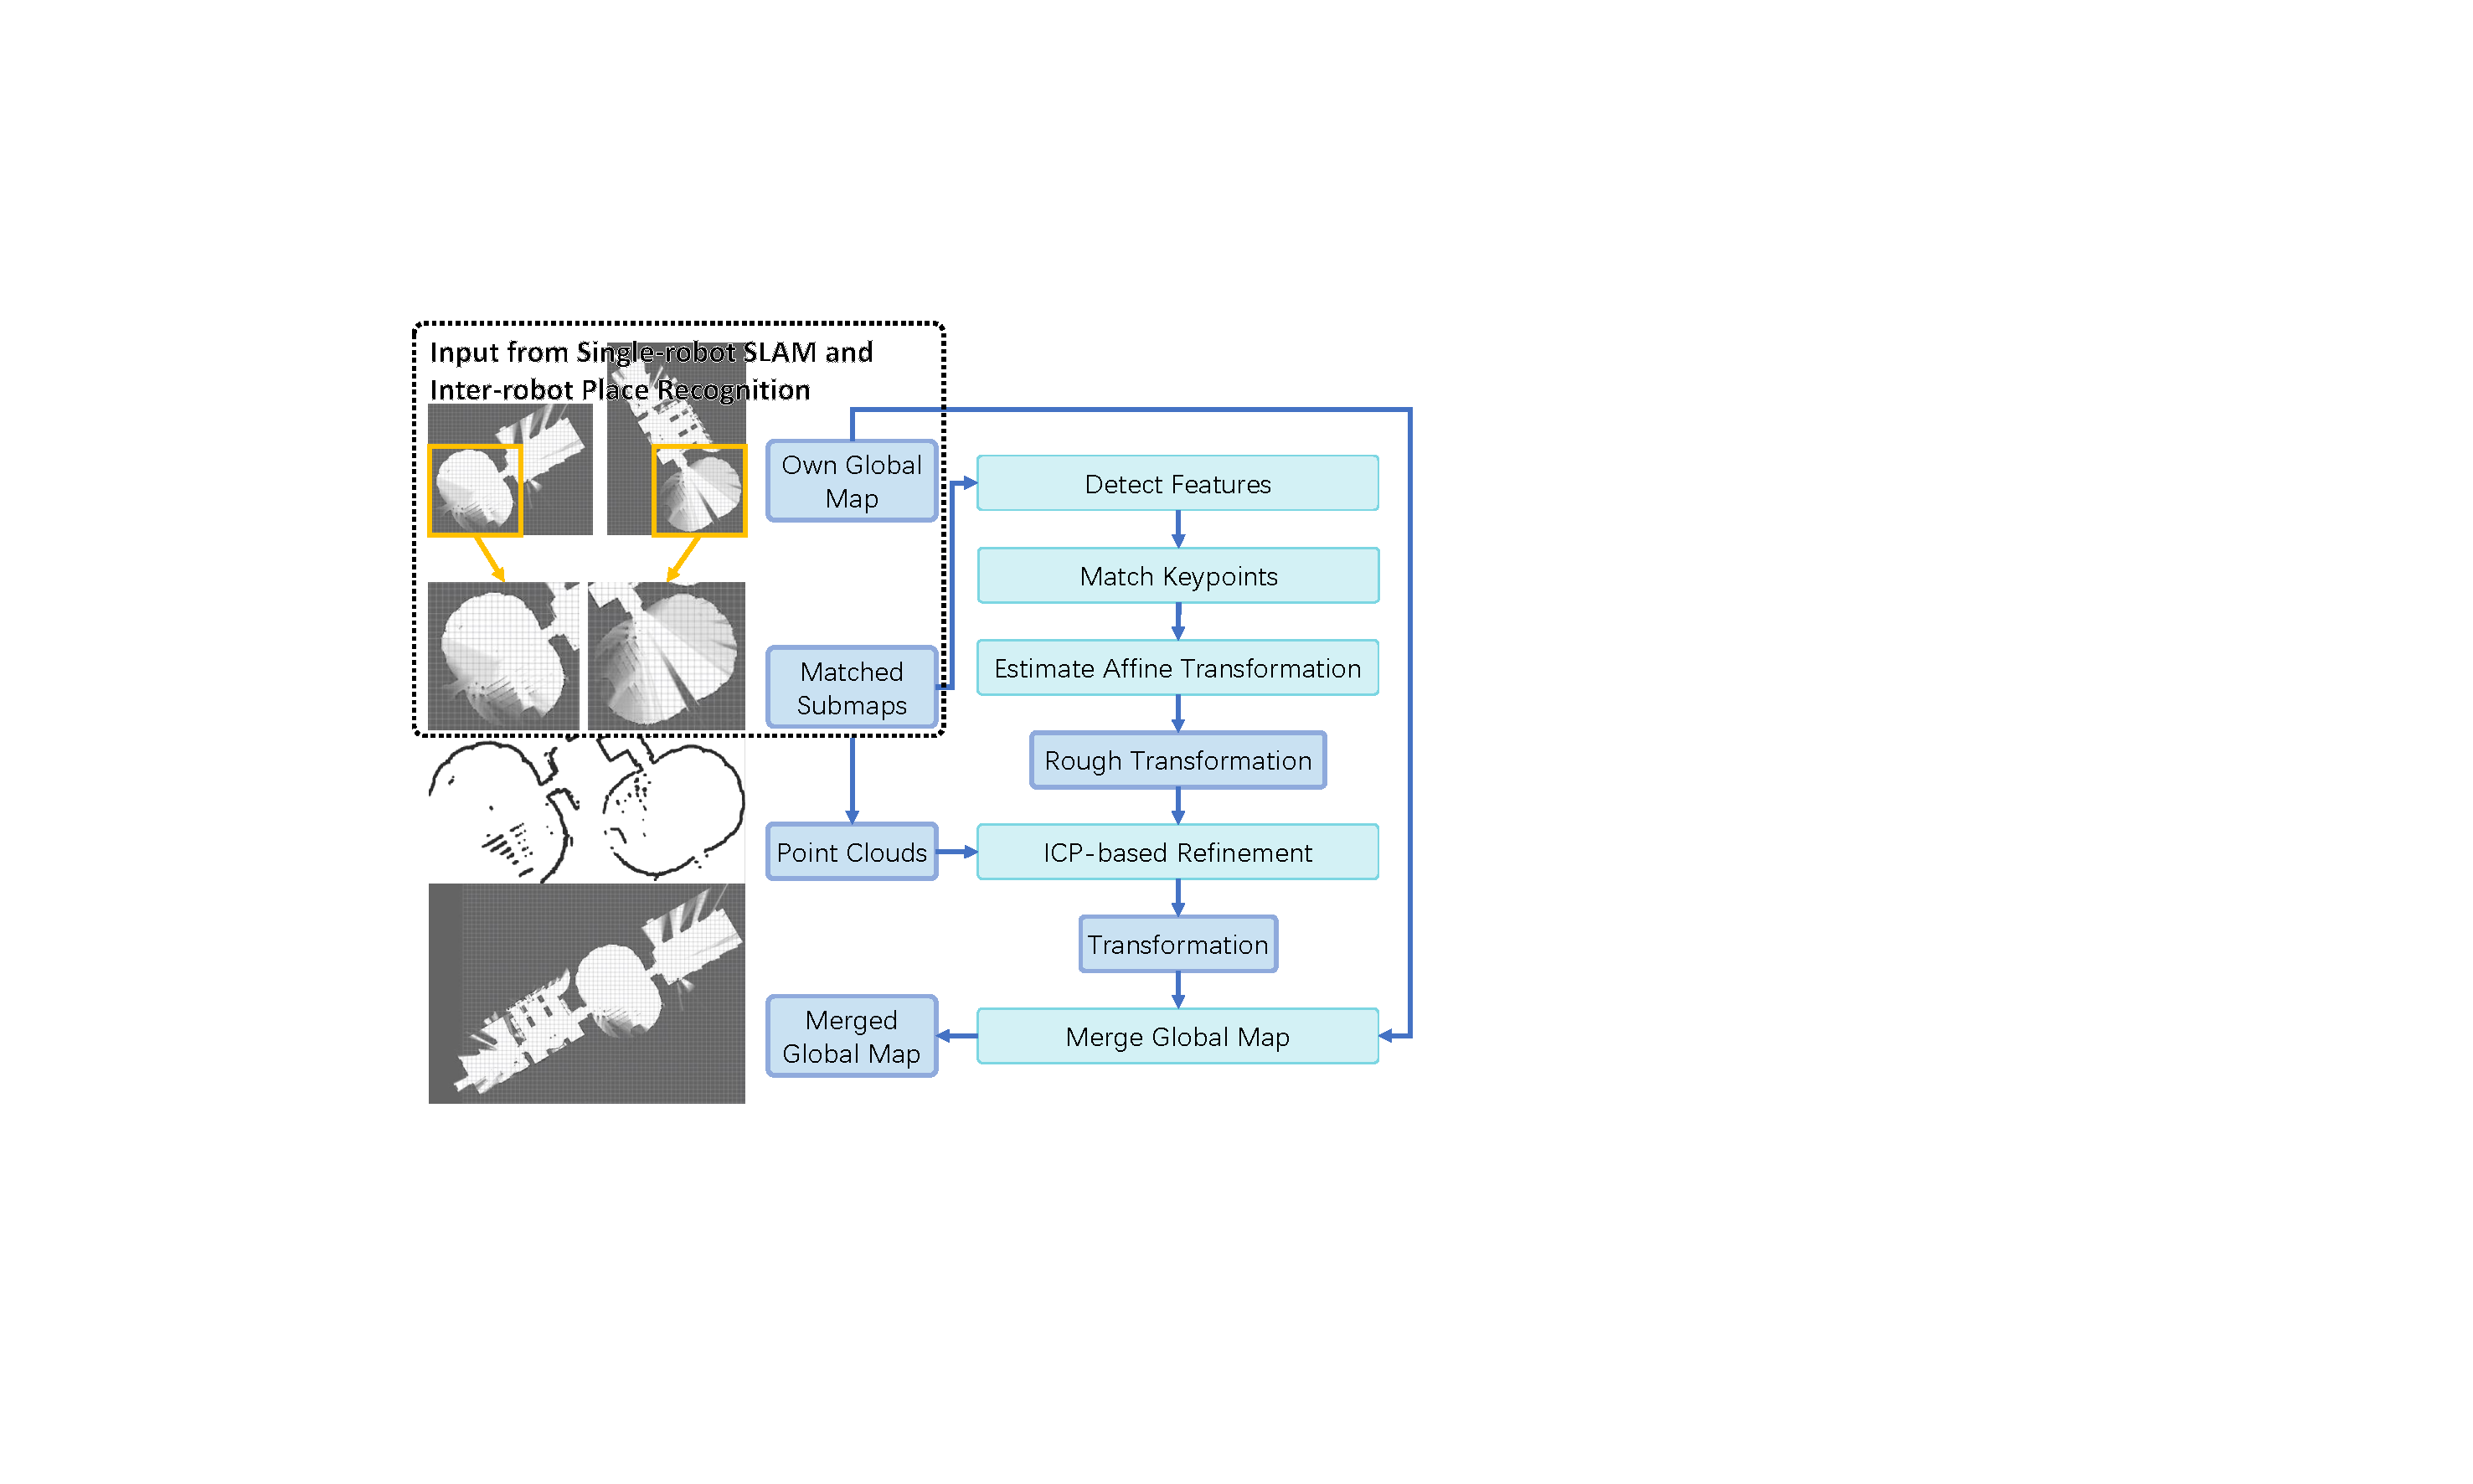
\includegraphics[width=0.99\linewidth]{fig/registration.pdf}
    \caption{An overview of the proposed method for relative pose estimation and map merging.}
    \label{fig:registration}
\end{figure}

We extract image-based features from submap and perform coarse registration. 
After that, we convert the submap to the point cloud and refine the registration result.
Firstly, we extract image-based features like AKAZE, ORB, SURF, etc.
We use the features matcher which finds two best matches for each feature and leaves the best one only if the ratio between descriptor distances is greater than the threshold.
And we check the geometric consistency of the matching results and delete incorrect matches.
After that, the inter-robot transformation can be estimated as the initial value of ICP.
Submaps are converted into point clouds for the refinement of the registration result based on ICP.
The map merger merges the own global maps according to the registration results to obtain the merged global map.